\documentclass[1p]{elsarticle_modified}
%\bibliographystyle{elsarticle-num}

%\usepackage[colorlinks]{hyperref}
%\usepackage{abbrmath_seonhwa} %\Abb, \Ascr, \Acal ,\Abf, \Afrak
\usepackage{amsfonts}
\usepackage{amssymb}
\usepackage{amsmath}
\usepackage{amsthm}
\usepackage{scalefnt}
\usepackage{amsbsy}
\usepackage{kotex}
\usepackage{caption}
\usepackage{subfig}
\usepackage{color}
\usepackage{graphicx}
\usepackage{xcolor} %% white, black, red, green, blue, cyan, magenta, yellow
\usepackage{float}
\usepackage{setspace}
\usepackage{hyperref}

\usepackage{tikz}
\usetikzlibrary{arrows}

\usepackage{multirow}
\usepackage{array} % fixed length table
\usepackage{hhline}

%%%%%%%%%%%%%%%%%%%%%
\makeatletter
\renewcommand*\env@matrix[1][\arraystretch]{%
	\edef\arraystretch{#1}%
	\hskip -\arraycolsep
	\let\@ifnextchar\new@ifnextchar
	\array{*\c@MaxMatrixCols c}}
\makeatother %https://tex.stackexchange.com/questions/14071/how-can-i-increase-the-line-spacing-in-a-matrix
%%%%%%%%%%%%%%%

\usepackage[normalem]{ulem}

\newcommand{\msout}[1]{\ifmmode\text{\sout{\ensuremath{#1}}}\else\sout{#1}\fi}
%SOURCE: \msout is \stkout macro in https://tex.stackexchange.com/questions/20609/strikeout-in-math-mode

\newcommand{\cancel}[1]{
	\ifmmode
	{\color{red}\msout{#1}}
	\else
	{\color{red}\sout{#1}}
	\fi
}

\newcommand{\add}[1]{
	{\color{blue}\uwave{#1}}
}

\newcommand{\replace}[2]{
	\ifmmode
	{\color{red}\msout{#1}}{\color{blue}\uwave{#2}}
	\else
	{\color{red}\sout{#1}}{\color{blue}\uwave{#2}}
	\fi
}

\newcommand{\Sol}{\mathcal{S}} %segment
\newcommand{\D}{D} %diagram
\newcommand{\A}{\mathcal{A}} %arc


%%%%%%%%%%%%%%%%%%%%%%%%%%%%%5 test

\def\sl{\operatorname{\textup{SL}}(2,\Cbb)}
\def\psl{\operatorname{\textup{PSL}}(2,\Cbb)}
\def\quan{\mkern 1mu \triangleright \mkern 1mu}

\theoremstyle{definition}
\newtheorem{thm}{Theorem}[section]
\newtheorem{prop}[thm]{Proposition}
\newtheorem{lem}[thm]{Lemma}
\newtheorem{ques}[thm]{Question}
\newtheorem{cor}[thm]{Corollary}
\newtheorem{defn}[thm]{Definition}
\newtheorem{exam}[thm]{Example}
\newtheorem{rmk}[thm]{Remark}
\newtheorem{alg}[thm]{Algorithm}

\newcommand{\I}{\sqrt{-1}}
\begin{document}

%\begin{frontmatter}
%
%\title{Boundary parabolic representations of knots up to 8 crossings}
%
%%% Group authors per affiliation:
%\author{Yunhi Cho} 
%\address{Department of Mathematics, University of Seoul, Seoul, Korea}
%\ead{yhcho@uos.ac.kr}
%
%
%\author{Seonhwa Kim} %\fnref{s_kim}}
%\address{Center for Geometry and Physics, Institute for Basic Science, Pohang, 37673, Korea}
%\ead{ryeona17@ibs.re.kr}
%
%\author{Hyuk Kim}
%\address{Department of Mathematical Sciences, Seoul National University, Seoul 08826, Korea}
%\ead{hyukkim@snu.ac.kr}
%
%\author{Seokbeom Yoon}
%\address{Department of Mathematical Sciences, Seoul National University, Seoul, 08826,  Korea}
%\ead{sbyoon15@snu.ac.kr}
%
%\begin{abstract}
%We find all boundary parabolic representation of knots up to 8 crossings.
%
%\end{abstract}
%\begin{keyword}
%    \MSC[2010] 57M25 
%\end{keyword}
%
%\end{frontmatter}

%\linenumbers
%\tableofcontents
%
\newcommand\colored[1]{\textcolor{white}{\rule[-0.35ex]{0.8em}{1.4ex}}\kern-0.8em\color{red} #1}%
%\newcommand\colored[1]{\textcolor{white}{ #1}\kern-2.17ex	\textcolor{white}{ #1}\kern-1.81ex	\textcolor{white}{ #1}\kern-2.15ex\color{red}#1	}

{\Large $\underline{9_{43}~(K9n_{3})}$}

\setlength{\tabcolsep}{10pt}
\renewcommand{\arraystretch}{1.6}
\vspace{1cm}\begin{tabular}{m{100pt}>{\centering\arraybackslash}m{274pt}}
\multirow{5}{120pt}{
	\centering
	\includegraphics[width=112pt]{../../../GIT/diagram.site/Diagrams/png/78_9_43.png}\\
\ \ \ A knot diagram\footnotemark}&
\allowdisplaybreaks
\textbf{Linearized knot diagam} \\
\cline{2-2}
 &
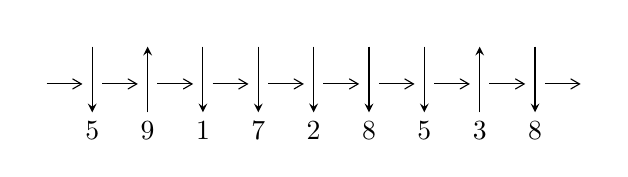
\begin{tikzpicture}[x=20pt, y=17pt]
	% nodes
	\node (C0) at (0, 0) {};
	\node (C1) at (1, 0) {};
	\node (C1U) at (1, +1) {};
	\node (C1D) at (1, -1) {5};

	\node (C2) at (2, 0) {};
	\node (C2U) at (2, +1) {};
	\node (C2D) at (2, -1) {9};

	\node (C3) at (3, 0) {};
	\node (C3U) at (3, +1) {};
	\node (C3D) at (3, -1) {1};

	\node (C4) at (4, 0) {};
	\node (C4U) at (4, +1) {};
	\node (C4D) at (4, -1) {7};

	\node (C5) at (5, 0) {};
	\node (C5U) at (5, +1) {};
	\node (C5D) at (5, -1) {2};

	\node (C6) at (6, 0) {};
	\node (C6U) at (6, +1) {};
	\node (C6D) at (6, -1) {8};

	\node (C7) at (7, 0) {};
	\node (C7U) at (7, +1) {};
	\node (C7D) at (7, -1) {5};

	\node (C8) at (8, 0) {};
	\node (C8U) at (8, +1) {};
	\node (C8D) at (8, -1) {3};

	\node (C9) at (9, 0) {};
	\node (C9U) at (9, +1) {};
	\node (C9D) at (9, -1) {8};
	\node (C10) at (10, 0) {};

	% arrows
	\draw[->,>={angle 60}]
	(C0) edge (C1) (C1) edge (C2) (C2) edge (C3) (C3) edge (C4) (C4) edge (C5) (C5) edge (C6) (C6) edge (C7) (C7) edge (C8) (C8) edge (C9) (C9) edge (C10) ;	\draw[->,>=stealth]
	(C1U) edge (C1D) (C2D) edge (C2U) (C3U) edge (C3D) (C4U) edge (C4D) (C5U) edge (C5D) (C6U) edge (C6D) (C7U) edge (C7D) (C8D) edge (C8U) (C9U) edge (C9D) ;
	\end{tikzpicture} \\
\hhline{~~} \\& 
\textbf{Solving Sequence} \\ \cline{2-2} 
 &
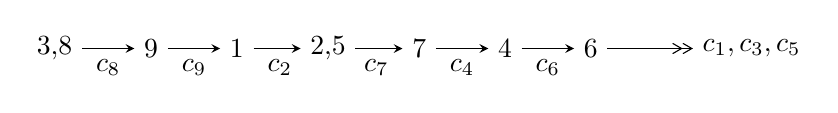
\begin{tikzpicture}[x=31pt, y=7pt]
	% node
	\node (A0) at (-1/8, 0) {3,8};
	\node (A1) at (1, 0) {9};
	\node (A2) at (2, 0) {1};
	\node (A3) at (49/16, 0) {2,5};
	\node (A4) at (33/8, 0) {7};
	\node (A5) at (41/8, 0) {4};
	\node (A6) at (49/8, 0) {6};
	\node (C1) at (1/2, -1) {$c_{8}$};
	\node (C2) at (3/2, -1) {$c_{9}$};
	\node (C3) at (5/2, -1) {$c_{2}$};
	\node (C4) at (29/8, -1) {$c_{7}$};
	\node (C5) at (37/8, -1) {$c_{4}$};
	\node (C6) at (45/8, -1) {$c_{6}$};
	\node (A7) at (8, 0) {$c_{1},c_{3},c_{5}$};

	% edge
	\draw[->,>=stealth]	
	(A0) edge (A1) (A1) edge (A2) (A2) edge (A3) (A3) edge (A4) (A4) edge (A5) (A5) edge (A6) ;
	\draw[->>,>={angle 60}]	
	(A6) edge (A7);
\end{tikzpicture} \\ 

\end{tabular} \\

\footnotetext{
The image of knot diagram is generated by the software ``\textbf{Draw programme}" developed by Andrew Bartholomew(\url{http://www.layer8.co.uk/maths/draw/index.htm\#Running-draw}), where we modified some parts for our purpose(\url{https://github.com/CATsTAILs/LinksPainter}).
}\phantom \\ \newline 
\centering \textbf{Ideals for irreducible components\footnotemark of $X_{\text{par}}$} 
 
\begin{align*}
I^u_{1}&=\langle 
- u^5+u^4-2 u^3+u^2+b- u+1,\;u^7-2 u^6+5 u^5-5 u^4+6 u^3-5 u^2+a+3 u-3,\\
\phantom{I^u_{1}}&\phantom{= \langle  }u^8-2 u^7+5 u^6-6 u^5+7 u^4-7 u^3+4 u^2-4 u+1\rangle \\
I^u_{2}&=\langle 
b+1,\;a- u-1,\;u^2+u+1\rangle \\
\\
\end{align*}
\raggedright * 2 irreducible components of $\dim_{\mathbb{C}}=0$, with total 10 representations.\\
\footnotetext{All coefficients of polynomials are rational numbers. But the coefficients are sometimes approximated in decimal forms when there is not enough margin.}
\newpage
\renewcommand{\arraystretch}{1}
\centering \section*{I. $I^u_{1}= \langle - u^5+u^4-2 u^3+u^2+b- u+1,\;u^7-2 u^6+5 u^5-5 u^4+6 u^3-5 u^2+a+3 u-3,\;u^8-2 u^7+\cdots-4 u+1 \rangle$}
\flushleft \textbf{(i) Arc colorings}\\
\begin{tabular}{m{7pt} m{180pt} m{7pt} m{180pt} }
\flushright $a_{3}=$&$\begin{pmatrix}0\\u\end{pmatrix}$ \\
\flushright $a_{8}=$&$\begin{pmatrix}1\\0\end{pmatrix}$ \\
\flushright $a_{9}=$&$\begin{pmatrix}1\\- u^2\end{pmatrix}$ \\
\flushright $a_{1}=$&$\begin{pmatrix}u^2+1\\- u^2\end{pmatrix}$ \\
\flushright $a_{2}=$&$\begin{pmatrix}- u\\u^3+u\end{pmatrix}$ \\
\flushright $a_{5}=$&$\begin{pmatrix}- u^7+2 u^6-5 u^5+5 u^4-6 u^3+5 u^2-3 u+3\\u^5- u^4+2 u^3- u^2+u-1\end{pmatrix}$ \\
\flushright $a_{7}=$&$\begin{pmatrix}- u^7+2 u^6-4 u^5+5 u^4-4 u^3+5 u^2-2 u+3\\- u^6+u^5-3 u^4+2 u^3-2 u^2+2 u-1\end{pmatrix}$ \\
\flushright $a_{4}=$&$\begin{pmatrix}u^5+2 u^3+u\\- u^5- u^3- u\end{pmatrix}$ \\
\flushright $a_{6}=$&$\begin{pmatrix}- u^7+u^6-3 u^5+2 u^4-2 u^3+3 u^2+2\\- u^6+u^5-3 u^4+2 u^3-2 u^2+2 u-1\end{pmatrix}$\\ \flushright $a_{6}=$&$\begin{pmatrix}- u^7+u^6-3 u^5+2 u^4-2 u^3+3 u^2+2\\- u^6+u^5-3 u^4+2 u^3-2 u^2+2 u-1\end{pmatrix}$\\&\end{tabular}
\flushleft \textbf{(ii) Obstruction class $= -1$}\\~\\
\flushleft \textbf{(iii) Cusp Shapes $= - u^7+u^6- u^5-2 u^4+6 u^3-5 u^2+5 u-10$}\\~\\
\newpage\renewcommand{\arraystretch}{1}
\flushleft \textbf{(iv) u-Polynomials at the component}\newline \\
\begin{tabular}{m{50pt}|m{274pt}}
Crossings & \hspace{64pt}u-Polynomials at each crossing \\
\hline $$\begin{aligned}c_{1},c_{5}\end{aligned}$$&$\begin{aligned}
&u^8+u^7-7 u^6-4 u^5+16 u^4-3 u^3-9 u^2-8 u-4
\end{aligned}$\\
\hline $$\begin{aligned}c_{2},c_{8}\end{aligned}$$&$\begin{aligned}
&u^8+2 u^7+5 u^6+6 u^5+7 u^4+7 u^3+4 u^2+4 u+1
\end{aligned}$\\
\hline $$\begin{aligned}c_{3}\end{aligned}$$&$\begin{aligned}
&u^8-2 u^7-7 u^6+12 u^5+5 u^4+3 u^3-2 u^2+2 u+1
\end{aligned}$\\
\hline $$\begin{aligned}c_{4},c_{7}\end{aligned}$$&$\begin{aligned}
&u^8-3 u^7-2 u^6+9 u^5+5 u^4-13 u^3-3 u^2+3 u-1
\end{aligned}$\\
\hline $$\begin{aligned}c_{6}\end{aligned}$$&$\begin{aligned}
&u^8+13 u^7+68 u^6+185 u^5+287 u^4+249 u^3+77 u^2+3 u+1
\end{aligned}$\\
\hline $$\begin{aligned}c_{9}\end{aligned}$$&$\begin{aligned}
&u^8+6 u^7+15 u^6+14 u^5-9 u^4-31 u^3-26 u^2-8 u+1
\end{aligned}$\\
\hline
\end{tabular}\\~\\
\newpage\renewcommand{\arraystretch}{1}
\flushleft \textbf{(v) Riley Polynomials at the component}\newline \\
\begin{tabular}{m{50pt}|m{274pt}}
Crossings & \hspace{64pt}Riley Polynomials at each crossing \\
\hline $$\begin{aligned}c_{1},c_{5}\end{aligned}$$&$\begin{aligned}
&y^8-15 y^7+89 y^6-252 y^5+366 y^4-305 y^3-95 y^2+8 y+16
\end{aligned}$\\
\hline $$\begin{aligned}c_{2},c_{8}\end{aligned}$$&$\begin{aligned}
&y^8+6 y^7+15 y^6+14 y^5-9 y^4-31 y^3-26 y^2-8 y+1
\end{aligned}$\\
\hline $$\begin{aligned}c_{3}\end{aligned}$$&$\begin{aligned}
&y^8-18 y^7+107 y^6-206 y^5-9 y^4-91 y^3+2 y^2-8 y+1
\end{aligned}$\\
\hline $$\begin{aligned}c_{4},c_{7}\end{aligned}$$&$\begin{aligned}
&y^8-13 y^7+68 y^6-185 y^5+287 y^4-249 y^3+77 y^2-3 y+1
\end{aligned}$\\
\hline $$\begin{aligned}c_{6}\end{aligned}$$&$\begin{aligned}
&y^8-33 y^7+\cdots+145 y+1
\end{aligned}$\\
\hline $$\begin{aligned}c_{9}\end{aligned}$$&$\begin{aligned}
&y^8-6 y^7+39 y^6-146 y^5+267 y^4-239 y^3+162 y^2-116 y+1
\end{aligned}$\\
\hline
\end{tabular}\\~\\
\newpage\flushleft \textbf{(vi) Complex Volumes and Cusp Shapes}
$$\begin{array}{c|c|c}  
\text{Solutions to }I^u_{1}& \I (\text{vol} + \sqrt{-1}CS) & \text{Cusp shape}\\
 \hline 
\begin{aligned}
u &= -0.381025 + 0.877247 I \\
a &= \phantom{-}0.332599 + 0.127423 I \\
b &= \phantom{-}0.238510 - 0.243220 I\end{aligned}
 & -0.36340 - 1.66195 I & -2.61632 + 3.48117 I \\ \hline\begin{aligned}
u &= -0.381025 - 0.877247 I \\
a &= \phantom{-}0.332599 - 0.127423 I \\
b &= \phantom{-}0.238510 + 0.243220 I\end{aligned}
 & -0.36340 + 1.66195 I & -2.61632 - 3.48117 I \\ \hline\begin{aligned}
u &= \phantom{-}1.11498\phantom{ +0.000000I} \\
a &= -1.63389\phantom{ +0.000000I} \\
b &= \phantom{-}1.82176\phantom{ +0.000000I}\end{aligned}
 & -11.0713\phantom{ +0.000000I} & -7.35940\phantom{ +0.000000I} \\ \hline\begin{aligned}
u &= \phantom{-}0.126694 + 1.193160 I \\
a &= -0.399095 - 1.030330 I \\
b &= -1.178780 + 0.606721 I\end{aligned}
 & -4.43209 + 1.62541 I & -10.58501 - 1.42555 I \\ \hline\begin{aligned}
u &= \phantom{-}0.126694 - 1.193160 I \\
a &= -0.399095 + 1.030330 I \\
b &= -1.178780 - 0.606721 I\end{aligned}
 & -4.43209 - 1.62541 I & -10.58501 + 1.42555 I \\ \hline\begin{aligned}
u &= \phantom{-}0.54402 + 1.39007 I \\
a &= -0.321827 + 1.239280 I \\
b &= \phantom{-}1.89776 - 0.22684 I\end{aligned}
 & -15.4360 + 5.9041 I & -9.72541 - 2.82977 I \\ \hline\begin{aligned}
u &= \phantom{-}0.54402 - 1.39007 I \\
a &= -0.321827 - 1.239280 I \\
b &= \phantom{-}1.89776 + 0.22684 I\end{aligned}
 & -15.4360 - 5.9041 I & -9.72541 + 2.82977 I \\ \hline\begin{aligned}
u &= \phantom{-}0.305633\phantom{ +0.000000I} \\
a &= \phantom{-}2.41054\phantom{ +0.000000I} \\
b &= -0.736738\phantom{ +0.000000I}\end{aligned}
 & -1.10361\phantom{ +0.000000I} & -8.78710\phantom{ +0.000000I}\\
 \hline 
 \end{array}$$\newpage\newpage\renewcommand{\arraystretch}{1}
\centering \section*{II. $I^u_{2}= \langle b+1,\;a- u-1,\;u^2+u+1 \rangle$}
\flushleft \textbf{(i) Arc colorings}\\
\begin{tabular}{m{7pt} m{180pt} m{7pt} m{180pt} }
\flushright $a_{3}=$&$\begin{pmatrix}0\\u\end{pmatrix}$ \\
\flushright $a_{8}=$&$\begin{pmatrix}1\\0\end{pmatrix}$ \\
\flushright $a_{9}=$&$\begin{pmatrix}1\\u+1\end{pmatrix}$ \\
\flushright $a_{1}=$&$\begin{pmatrix}- u\\u+1\end{pmatrix}$ \\
\flushright $a_{2}=$&$\begin{pmatrix}- u\\u+1\end{pmatrix}$ \\
\flushright $a_{5}=$&$\begin{pmatrix}u+1\\-1\end{pmatrix}$ \\
\flushright $a_{7}=$&$\begin{pmatrix}u+2\\-1\end{pmatrix}$ \\
\flushright $a_{4}=$&$\begin{pmatrix}-1\\0\end{pmatrix}$ \\
\flushright $a_{6}=$&$\begin{pmatrix}u+1\\-1\end{pmatrix}$\\ \flushright $a_{6}=$&$\begin{pmatrix}u+1\\-1\end{pmatrix}$\\&\end{tabular}
\flushleft \textbf{(ii) Obstruction class $= 1$}\\~\\
\flushleft \textbf{(iii) Cusp Shapes $= 4 u-7$}\\~\\
\newpage\renewcommand{\arraystretch}{1}
\flushleft \textbf{(iv) u-Polynomials at the component}\newline \\
\begin{tabular}{m{50pt}|m{274pt}}
Crossings & \hspace{64pt}u-Polynomials at each crossing \\
\hline $$\begin{aligned}c_{1},c_{5}\end{aligned}$$&$\begin{aligned}
&u^2
\end{aligned}$\\
\hline $$\begin{aligned}c_{2}\end{aligned}$$&$\begin{aligned}
&u^2- u+1
\end{aligned}$\\
\hline $$\begin{aligned}c_{3},c_{8},c_{9}\end{aligned}$$&$\begin{aligned}
&u^2+u+1
\end{aligned}$\\
\hline $$\begin{aligned}c_{4},c_{6}\end{aligned}$$&$\begin{aligned}
&(u-1)^2
\end{aligned}$\\
\hline $$\begin{aligned}c_{7}\end{aligned}$$&$\begin{aligned}
&(u+1)^2
\end{aligned}$\\
\hline
\end{tabular}\\~\\
\newpage\renewcommand{\arraystretch}{1}
\flushleft \textbf{(v) Riley Polynomials at the component}\newline \\
\begin{tabular}{m{50pt}|m{274pt}}
Crossings & \hspace{64pt}Riley Polynomials at each crossing \\
\hline $$\begin{aligned}c_{1},c_{5}\end{aligned}$$&$\begin{aligned}
&y^2
\end{aligned}$\\
\hline $$\begin{aligned}c_{2},c_{3},c_{8}\\c_{9}\end{aligned}$$&$\begin{aligned}
&y^2+y+1
\end{aligned}$\\
\hline $$\begin{aligned}c_{4},c_{6},c_{7}\end{aligned}$$&$\begin{aligned}
&(y-1)^2
\end{aligned}$\\
\hline
\end{tabular}\\~\\
\newpage\flushleft \textbf{(vi) Complex Volumes and Cusp Shapes}
$$\begin{array}{c|c|c}  
\text{Solutions to }I^u_{2}& \I (\text{vol} + \sqrt{-1}CS) & \text{Cusp shape}\\
 \hline 
\begin{aligned}
u &= -0.500000 + 0.866025 I \\
a &= \phantom{-}0.500000 + 0.866025 I \\
b &= -1.00000\phantom{ +0.000000I}\end{aligned}
 & -1.64493 - 2.02988 I & -9.00000 + 3.46410 I \\ \hline\begin{aligned}
u &= -0.500000 - 0.866025 I \\
a &= \phantom{-}0.500000 - 0.866025 I \\
b &= -1.00000\phantom{ +0.000000I}\end{aligned}
 & -1.64493 + 2.02988 I & -9.00000 - 3.46410 I\\
 \hline 
 \end{array}$$\newpage
\newpage\renewcommand{\arraystretch}{1}
\centering \section*{ III. u-Polynomials}
\begin{tabular}{m{50pt}|m{274pt}}
Crossings & \hspace{64pt}u-Polynomials at each crossing \\
\hline $$\begin{aligned}c_{1},c_{5}\end{aligned}$$&$\begin{aligned}
&u^2(u^8+u^7-7 u^6-4 u^5+16 u^4-3 u^3-9 u^2-8 u-4)
\end{aligned}$\\
\hline $$\begin{aligned}c_{2}\end{aligned}$$&$\begin{aligned}
&(u^2- u+1)(u^8+2 u^7+5 u^6+6 u^5+7 u^4+7 u^3+4 u^2+4 u+1)
\end{aligned}$\\
\hline $$\begin{aligned}c_{3}\end{aligned}$$&$\begin{aligned}
&(u^2+u+1)(u^8-2 u^7-7 u^6+12 u^5+5 u^4+3 u^3-2 u^2+2 u+1)
\end{aligned}$\\
\hline $$\begin{aligned}c_{4}\end{aligned}$$&$\begin{aligned}
&(u-1)^2(u^8-3 u^7-2 u^6+9 u^5+5 u^4-13 u^3-3 u^2+3 u-1)
\end{aligned}$\\
\hline $$\begin{aligned}c_{6}\end{aligned}$$&$\begin{aligned}
&((u-1)^2)(u^8+13 u^7+\cdots+3 u+1)
\end{aligned}$\\
\hline $$\begin{aligned}c_{7}\end{aligned}$$&$\begin{aligned}
&(u+1)^2(u^8-3 u^7-2 u^6+9 u^5+5 u^4-13 u^3-3 u^2+3 u-1)
\end{aligned}$\\
\hline $$\begin{aligned}c_{8}\end{aligned}$$&$\begin{aligned}
&(u^2+u+1)(u^8+2 u^7+5 u^6+6 u^5+7 u^4+7 u^3+4 u^2+4 u+1)
\end{aligned}$\\
\hline $$\begin{aligned}c_{9}\end{aligned}$$&$\begin{aligned}
&(u^2+u+1)(u^8+6 u^7+15 u^6+14 u^5-9 u^4-31 u^3-26 u^2-8 u+1)
\end{aligned}$\\
\hline
\end{tabular}\newpage\renewcommand{\arraystretch}{1}
\centering \section*{ IV. Riley Polynomials}
\begin{tabular}{m{50pt}|m{274pt}}
Crossings & \hspace{64pt}Riley Polynomials at each crossing \\
\hline $$\begin{aligned}c_{1},c_{5}\end{aligned}$$&$\begin{aligned}
&y^2(y^8-15 y^7+89 y^6-252 y^5+366 y^4-305 y^3-95 y^2+8 y+16)
\end{aligned}$\\
\hline $$\begin{aligned}c_{2},c_{8}\end{aligned}$$&$\begin{aligned}
&(y^2+y+1)(y^8+6 y^7+15 y^6+14 y^5-9 y^4-31 y^3-26 y^2-8 y+1)
\end{aligned}$\\
\hline $$\begin{aligned}c_{3}\end{aligned}$$&$\begin{aligned}
&(y^2+y+1)(y^8-18 y^7+\cdots-8 y+1)
\end{aligned}$\\
\hline $$\begin{aligned}c_{4},c_{7}\end{aligned}$$&$\begin{aligned}
&((y-1)^2)(y^8-13 y^7+\cdots-3 y+1)
\end{aligned}$\\
\hline $$\begin{aligned}c_{6}\end{aligned}$$&$\begin{aligned}
&((y-1)^2)(y^8-33 y^7+\cdots+145 y+1)
\end{aligned}$\\
\hline $$\begin{aligned}c_{9}\end{aligned}$$&$\begin{aligned}
&(y^2+y+1)\\
&\cdot(y^8-6 y^7+39 y^6-146 y^5+267 y^4-239 y^3+162 y^2-116 y+1)
\end{aligned}$\\
\hline
\end{tabular}
\vskip 2pc
\end{document}